\chapter{Equations and Inequalities}

\section*{Equations}

Solve each equation. Round decimal answers to 2 decimal places.

\begin{multicols}{3}
\begin{enumerate}
	\item $-7x + 5 = -10x + 11$
	\item $\frac{2}{3}x - 10 = \frac{5}{8}$
	\item $-0.2x - 3(x+1.4) = -5.2x + 1$
\end{enumerate}	\setcounter{Review}{\value{enumi}}
\end{multicols}
\begin{multicols}{3}
\begin{enumerate}	\setcounter{enumi}{\value{Review}}
	\item $1.3 + 2.1(6.3x + 12) = -19.7$
	\item $\frac{1}{4}x + \frac{3}{7} = -2\left(x + \frac{3}{8}\right)$
\end{enumerate}	\setcounter{Review}{\value{enumi}}
\end{multicols}

Solve each for the variable indicated.

\begin{multicols}{3}
\begin{enumerate}	\setcounter{enumi}{\value{Review}}
	\item $F = ma; \text{ for } a$
	\item $PV = nRT; \text{ for } n$
	\item $m = \frac{y_2-y_1}{x_2-x_1}; \text{ for } y_2$
\end{enumerate}	\setcounter{Review}{\value{enumi}}
\end{multicols}
\begin{multicols}{3}
\begin{enumerate}	\setcounter{enumi}{\value{Review}}
	\item $m = \frac{y_2-y_1}{x_2-x_1}$; for $y_1$
    \item $v = v_0 + gt$; for $t$
    \item $S = 180(n-2)$; for $n$
\end{enumerate}	\setcounter{Review}{\value{enumi}}
\end{multicols}




\section*{Inequalities}

Solve each inequality. Graph your answers on a number line.

\begin{multicols}{3}
\begin{enumerate}
	\item $2(x+2) \leq 4x - 2(x-1)$
	\item $-3.2x - 5(x - 1.5) > 7.7 + 1.8x$
\end{enumerate}
\end{multicols}

\newpage

\section{Answer Key}

\subsection*{Equations}

\begin{multicols}{3}
\begin{enumerate}
	\item $x = 2$
	\item $x = \frac{255}{16}$
	\item $x = 2.6$
\end{enumerate}	\setcounter{Review}{\value{enumi}}
\end{multicols}
\begin{multicols}{3}
\begin{enumerate}	\setcounter{enumi}{\value{Review}}
	\item $x = -3.49$
	\item $x = -\frac{11}{21}$
\end{enumerate}	\setcounter{Review}{\value{enumi}}
\end{multicols}

\begin{multicols}{3}
\begin{enumerate}	\setcounter{enumi}{\value{Review}}
	\item $a = \frac{F}{m}$
	\item $n = \frac{PV}{RT}$
	\item $y_2 = m(x_2-x_1)+y_1$
\end{enumerate}	\setcounter{Review}{\value{enumi}}
\end{multicols}
\begin{multicols}{3}
\begin{enumerate}	\setcounter{enumi}{\value{Review}}
	\item $y_1 = y_2-m(x_2-x_1)$
    \item $t = \frac{v-v_0}{g}$
    \item $n = \frac{S}{180} + 2$
\end{enumerate}	\setcounter{Review}{\value{enumi}}
\end{multicols}


\subsection*{Inequalities}

\begin{multicols}{3}
\begin{enumerate}
	\item $\emptyset$		\newline\\
	\begin{tikzpicture}
	\draw[<->] (-2,0) -- (2,0);
	\end{tikzpicture}
	\item $x < -0.02$	\newline\\
	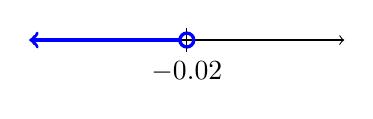
\begin{tikzpicture}
	\draw[<->] (-2,0) -- (2,0);
	\draw (0,0.15) -- (0,-0.15) node [below] {$-0.02$};
	\draw[->, very thick, blue, shorten <= 2.5pt] (0,0) -- (-2,0);
	\draw[blue, very thick] (0,0) circle [radius = 2.5pt];
	\end{tikzpicture}
\end{enumerate}
\end{multicols}